\section{Presentation}

For the demonstration of our project, we created a short video to show what our sonic art installation 'Moody Plant' actually does and how it works. You can see our video documentation on Youtube \cite{youtubeDemo}.

The plant was issued in the exhibition 'Union Reflection Assembly' by the degree program 'Communication, Sound and Interaction Design' at FH JOANNEUM in Graz. It got its main performance during the live stream of the vernissage on 27th February 2021, where it communicated with the moderators and even made it to Austria's public broadcasting ORF. For its big show we gave it the name 'Annabelle LaNoir'.


\begin{figure}[H]
\begin{center}
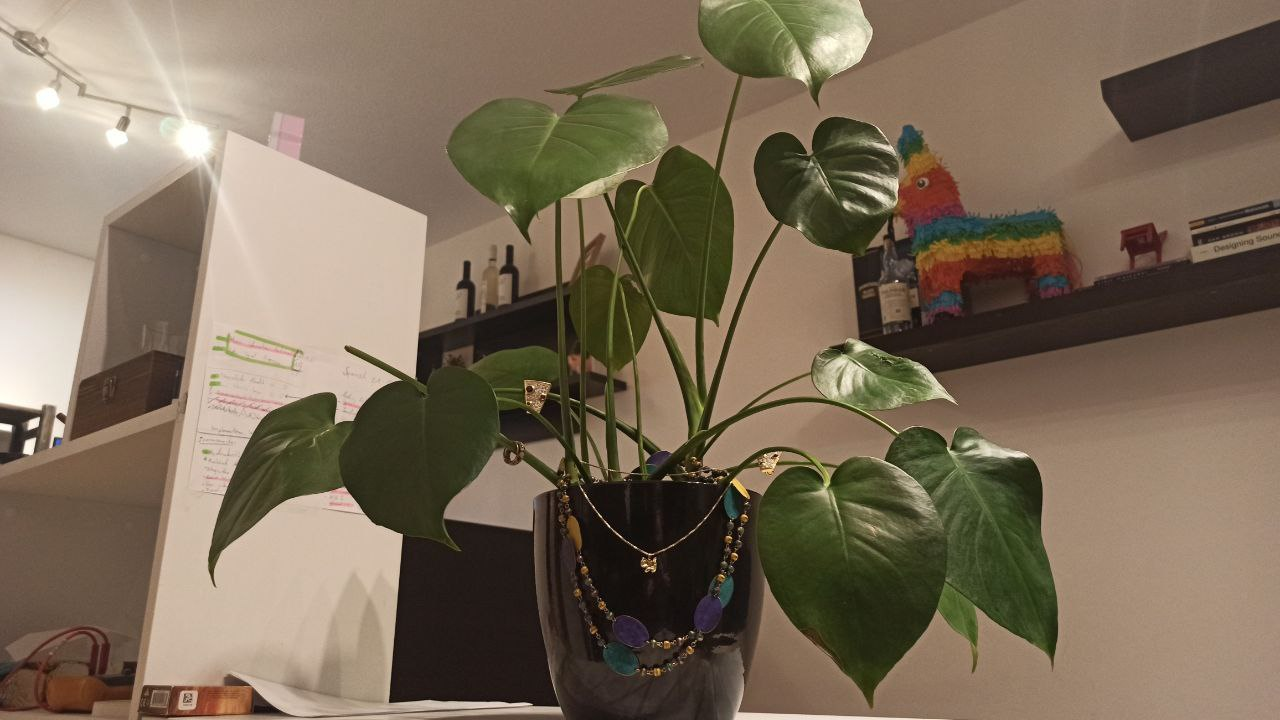
\includegraphics[width=0.8\linewidth]{Figures/plant2.jpg}
\caption{Moody Plant 'Annabelle LaNoire' dressed up for the big show}
\end{center}
\end{figure}



If you are interested, you can watch the live stream \cite{liveStream} of the vernissage, in which the affectionate plant has an appearance at 54:54. 
